\documentclass[10pt,a4paper]{article}

\usepackage[czech]{babel}
\usepackage[utf8]{inputenc}
\usepackage[T1]{fontenc}
\usepackage{graphicx}
\usepackage{float}
\usepackage{amsmath}
\usepackage{hyperref}
\usepackage{caption}
\usepackage{titlesec}
\usepackage{geometry}
\geometry{margin=1.5cm}
\usepackage{makecell}
\renewcommand\theadalign{bc}
\renewcommand\theadfont{\bfseries}
\renewcommand\theadgape{\Gape[1pt]}
\usepackage{algorithm}
\usepackage{algpseudocode}

\titleformat{\section}{\large\bfseries}{\thesection}{1em}{}
\titleformat{\subsection}{\normalsize\bfseries}{\thesubsection}{1em}{}

\title{\textbf{Závěrečná zpráva - Raytracer s akcelerační strukturou a implementací na GPU}}
\author{Jakub Votrubec \\
ČVUT FIT, NI-PG1 a NI-GPU 2024/25}
\date{}

\begin{document}

\maketitle

%================================================================================

\section{Úvod}

Tento dokument popisuje závěrečný výstup, v podobě semestrální práce, z předmětu NI-PG1 a NI-GPU. Náplní semestrální práce bylo vytvoření vlastního raytracering renderu, implementace akcelerační datové struktury pro zrychlení traverzace scény a následná implementace na GPU. Cílem bylo prokázat schopnost optimalizovat výkon raytraceru pomocí vhodné datové struktury a implementací na GPU.

Semestrální práce byla zpracována v jazyce C++, standard C++17, a využívá externí knihovny pouze pro načítání scén a konfigurace ve formátu \texttt{json}. Pro implementaci na GPU byl použit jazyk CUDA, který umožňuje efektivní paralelní zpracování dat na NVIDIA grafické kartě.

%================================================================================

\section{Definice problému}

Raytracing je technika v počítačové grafice, která simuluje šíření světla pro generování digitálních obrazů s vysokou vizuální věrností. Oproti rychlejším metodám, jako je scanline rendering, je ray tracing výpočetně náročnější, ale umožňuje realistické zobrazení optických jevů. Původně se používal hlavně pro statické obrázky a filmové vizuální efekty, kde nevadila delší doba renderování. Od roku 2018 je však díky hardwarové akceleraci možné využívat ray tracing i v reálném čase, například ve videohrách, často v kombinaci s tradičním rasterizačním vykreslováním. Ray tracing lze využít i pro simulaci zvukových vln, což umožňuje realističtější prostorový zvuk.

Funguje tak, že sleduje cestu paprsku z imaginárního oka skrz každý pixel obrazovky a vypočítává barvu objektu, který je v daném směru viditelný. Ray tracing předpokládá, že paprsek vždy protne zobrazovací rovinu. Po dosažení maximálního počtu odrazů nebo určité vzdálenosti bez průsečíku se výpočet pro daný paprsek ukončí a hodnota pixelu se aktualizuje. Pseudokód raytracingu jsem přiložil zde \ref{alg:raytracing}.

\begin{algorithm}[H]
\caption{Sekvenční raytracing}
\label{alg:raytracing}
\begin{algorithmic}[1]
    \State $O \gets$ objekty ve scéně
    \State $L \gets$ světla ve scéně
    \State $d_{\text{max}} \gets$ maximální hloubka zanoření
    \Function{trace\_ray}{Paprsek $r$, Hloubka $d$}
        \State $P \gets$ nejbližší průsečík $r$ a $o \in O$
        \If{$P$ neexistuje}
            \State \Return $barva\_pozadi$
        \EndIf
        \State $c \gets$ černá (počáteční barva)
        \ForAll{$l \in L$}
            \If{$l$ je vidět z $r.origin$}
                \State $c_l \gets$ výpočet barevného příspěvku z $l$ a $P$
                \State $c \gets c + c_l$
            \EndIf
        \EndFor
        \If{$d < d_{\text{max}}$}
            \State $c_r \gets$ \Call{trace\_ray}{odražený paprsek, $d+1$}
            \State $c_t \gets$ \Call{trace\_ray}{lomený paprsek, $d+1$}
            \State $c \gets + c_r + c_t$
        \EndIf
        \State \Return $c$
    \EndFunction
\end{algorithmic}
\end{algorithm}

%================================================================================

\section{Struktura raytraceru}

Implementoval jsem základní raytracer pro vykreslování scén složených z trojúhelníků. Raytracer nabízí následující funkce, mezi nimiž lze přepínat pomocí konfigurace:

\begin{itemize}
    \item Stíny pomocí stínových paprsků.
    \item Podpora plošného světla prostřednictvím náhodného vzorkování trojúhelníků.
    \item Vykreslení scény s různými osvětlovacími modely (distance shading, čistě difuzní osvětlení, Phongův a Blinn-Phongův osvětlovací model).
    \item Vykreslení scény s různými stínovacími modely (flat shading, smooth shading – Phongův stínací model).
    \item Podpora odrazu a lomu světla.
    \item Backface culling.
    \item Vykreslení scény s více vzorky na pixel (fuzzysampling), viz \textit{Použité metody nad rámec cvičení}~\ref{sec:used-methods}.
\end{itemize}

Raytracer je navržen tak, aby byl modulární a snadno rozšiřitelný. Hlavní třída \texttt{Raytracer} obsahuje metody pro vykreslování a ukládání výsledného obrazu. Scéna je reprezentována jako seznam trojúhelníků, které jsou načteny z~\texttt{.obj} souboru.

Raytracer načítá scénu pomocí knihovny \texttt{tinyobjloader} a používá knihovnu \texttt{nlohmann/json} pro načítání konfigurace. Výsledná scéna je vykreslena do formátu~\texttt{.ppm}.

\subsection{Použité metody nad rámec cvičení NI-PG1}
\label{sec:used-methods}

Při renderování scény jsem narazil na problém s velkým množstvím šumu ve výsledném obrazu, proto jsem se rozhodl implementovat vícenásobné vzorkování, které jsem nazval \textit{fuzzysampling}.

\textit{Fuzzysampling} spočívá v tom, že pro každý pixel se vygeneruje několik paprsků s mírně odlišným směrem. Jejich výsledky se následně průměrují, čímž se dosáhne hladšího obrazu a sníží se šum. Odchylky směru paprsku jsou generovány náhodně v rámci pixelu, což umožňuje zachovat detaily a zároveň eliminovat šum.

V rámci předmětu NI-GPU jsem implementoval raytracer na GPU pomocí jazyka CUDA. GPU verze raytraceru využívá stejnou datovou strukturu jako CPU verze, ale místo sekvenčního zpracování paprsků na CPU je využito paralelní zpracování na GPU. Každý paprsek je zpracován v samostatném vlákně, což umožňuje efektivní využití výpočetního výkonu GPU. Více viz \textit{Implementace na GPU}~\ref{sec:gpu-implementation}.

%================================================================================

\section{Akcelerační datová struktura}

Implementoval jsem dvě varianty akcelerační datové struktury octree:
\begin{itemize}
    \item základní varianta octree,
    \item parametrická varianta podle článku \textit{An Efficient Parametric Algorithm for Octree Traversal} od Revelles et al.
\end{itemize}

\subsection{Stavba a traverzace}

Octree je struktura, která dělí prostor na menší buňky, což umožňuje rychlejší vyhledávání kolizí mezi paprsky a trojúhelníky. Každý uzel octree obsahuje bounding box, který definuje prostor, který uzel pokrývá, a seznam trojúhelníků, které se v tomto prostoru nacházejí.

\subsubsection{Základní octree}

Základní octree je implementován jako rekurzivní struktura, která dělí prostor rekurzivně na osm dalších uzlů (oktetů), dokud není dosaženo maximální hloubky nebo počtu trojúhelníků v uzlu.

Traverzace probíhá tak, že pro každý paprsek se nejprve zjistí, zda protíná bounding box aktuálního uzlu. Pokud ano, poračuje se dál na jeho oktety, pokud ne, traverzace končí. Je-li oktet již list stromu (neobsahuje žádné vlastní oktety), traverzace končí a jeho trojúhelníky jsou přidány k výsledku. Traverzace pokračuje rekurzivně, dokud se neprohledá celý strom. Prochází se vždy všechny oktety uzlu.

\subsubsection{Parametrický octree}

Parametrický octree je vylepšená verze, která využívá parametrickou traverzaci. Tato metoda umožňuje efektivnější prohledávání prostoru tím, že využívá parametrické rovnice pro určení průsečíků paprsku s hranicemi uzlů octree (tzv. "slab" metoda).

Nejprve se vypočítají průsečíky paprsku s~hranicemi uzlu, z~nich se určí "čas", kdy paprsek vstoupí a~opustí daný uzel na jednotlivých osách. Pokud paprsek opustil uzel na nějaké ose dříve, nežli vstoupil na všech osách - minul bounding box uzlu a tato větev traverzace se uzavírá.

Pokud paprsek vstoupil, tak na základě průsečíku vstupu se vypočítá první oktet, do kterého paprsek vstoupí. Ten se následně přidá do fronty pro další zpracování. Následně se postupně projdou a přidají všechny oktety, do kterých paprsek vstoupí. Procházení všech dalších oktetů probíhá na základě konečného automatu, který určuje, do kterého oktetu paprsek vstoupí na základě jeho směru a aktuálního oktetu.

Optimalizace oproti základnímu octree spočívá v~tom, že se neprocházejí všechny oktety, ale pouze ty, do kterých paprsek skutečně vstoupí. Zároveň výpočet velikostí oktetů je založen jen na půlení velikosti rodičovského uzlu, což umožňuje efektivní a~výpočetně nenáročné dělení prostoru.

Parametrickou traverzaci se mi bohužel nepodařilo implementovat, více viz \textit{Problémy při implementaci}.

\subsection{Problémy při implementaci}

Při implementaci stavby octree jsem narazil na problémy s~přesností výpočtů velikosti oktetů. Kvůli chybě u datových typů s plovoucí desteinou čárkou se ne vždy přiřadily všechny trojúhelníky rodičovského uzlu do jeho oktetů, což vedlo k~chybám při traverzaci. Tento problém jsem vyřešil nafouknutím bounding boxů o toleranci \textit{epsilon}.

Bohužel se  mi nepodařilo správně implementovat a zprovoznit parametrický octree. Narazil na problémy při traverzaci. Traverzace nenalezne všechny trojúhelníky a scéna je poté vyrenderována s dírami, jak švýcarský sýr. Zkoušel jsem, jestli je problém opět v přesnosti výpočtů s čísly s plovoucí desetinnou čárkou, ale nepodařilo se mi ho vyřešit. Proto jsem se rozhodl parametrický octree nevyužít a~v~měření výkonu použít pouze základní octree.

%================================================================================

\section{Implementace na GPU}
\label{sec:gpu-implementation}

Implementace na GPU byla provedena pomocí jazyka CUDA. Hlavní myšlenkou bylo přesunout výpočet kolizí paprsků s trojúhelníky na GPU, což umožňuje paralelní zpracování velkého množství paprsků najednou.

GPU verze raytraceru využívá stejnou strukturu dat jako CPU verze, ale místo sekvenčního zpracování paprsků na CPU se využívá paralelní zpracování na GPU. Každý paprsek je zpracován v samostatném vlákně, což umožňuje efektivní využití výpočetního výkonu GPU.

\subsection{Implementace CPU vs GPU}

Při implementaci na GPU bylo nutné provést několik úprav oproti CPU verzi. Bylo potřeba odstranit závislost na standardní knihovně C++, alokovat paměť dostupnou pro GPU a přesunout data i nastavení rendereru do této alokované paměti. Struktura rendereru musela být změněna, protože funkce označené jako \texttt{\_\_global\_\_} nesmějí být členskými funkcemi tříd. Proto byly všechny GPU funkce přesunuty mimo třídu \texttt{Renderer} a funkce používané jak při CPU, tak GPU renderování byly zpřístupněny oběma přístupům. Dále bylo nutné některé funkce upravit tak, aby byly použitelné jak na CPU, tak na GPU, což bylo řešeno pomocí podmíněného překladu s direktivou \texttt{\#ifdef \_\_CUDA\_ARCH\_\_}.

Na GPU není implentována akcelerační struktura octree, ale pouze základní traverzace trojúhelníků. To znamená, že na GPU se nevyužívá žádná akcelerační datová struktura pro zrychlení traverzace scény. Všechny trojúhelníky jsou uloženy v~jednom poli a~pro každý paprsek se provádí sekvenční traverzace všech trojúhelníků.

Tato implementace je sice méně efektivní než CPU verze s octree, ale umožňuje využít paralelní zpracování na GPU a~dosáhnout tak vyššího výkonu při renderování scény.

Dále v GPU verzi není dostupná funkcionalita \textit{fuzzysampling}.

Implementaci na GPU lze nalést ve větvi \texttt{NI-GPU} v tomto repozitáři.

\subsection{Problémy při implementaci na GPU}

Při implementaci na GPU jsem narazil na problémy s tím, že funkce označené jako \texttt{\_\_global\_\_} nesmějí být členskými funkcemi tříd. To znamenalo, že jsem musel přesunout všechny GPU funkce mimo třídu \texttt{Renderer} a~přepsat je tak, aby byly použitelné jak na CPU, tak na GPU.

Dále jsem se potýkal s nečekaným problémem, co se týče generování náhodných čísel na GPU. Funkce \texttt{rand()} není dostupná v~CUDA, a tak jsem musel implementovat vlastní generátor náhodných čísel. Použil jsem jednoduchý lineární kongruentní generátor, který je dostatečný pro účely raytraceru.

%================================================================================

\section{Testování a měření výkonu}

\subsection{Nastavení měření}

Pro měření výkonu byla použita scéna \texttt{CornellBox-Sphere.obj} s následující konfigurací:

\begin{table}[H]
    \centering
    \caption{Použité nastavení rendereru}
    \begin{tabular}{|l|l|}
        \hline
        \thead{Parametr} & \thead{Hodnota} \\
        \hline
        Výsledné rozlišení & $800 \times 800$ \\
        \hline
        Max. zanoření paprsku & 10 \\
        \hline
        \makecell{Vzorků plošného světla \\ na trojúhelník} & 50 \\
        \hline
        Osvětlovací model & Blinn-Phong \\
        \hline
        Stínovací model & Smooth \\
        \hline
        Backface culling & Ano \\
        \hline
        Fuzzysampling & Ne \\
        \hline
    \end{tabular}
\end{table}

\begin{table}[H]
    \centering
    \caption{Použité nastavení struktury octree}
    \begin{tabular}{|l|c|}
        \hline
        \thead{Parametr} & \thead{Hodnota} \\
        \hline
        Max. počet trojúhelníků na uzel & 16 \\
        \hline
        Max. hloubka uzlů & 10 \\
        \hline
    \end{tabular}
\end{table}

\subsection{Výsledky měření}

Měření jsem prováděl na svém stroji \textit{Lenovo Legion} s následujícími parametry:

\begin{itemize}
    \item Procesor: AMD Ryzen 5 5600H; 3,3 GHz
    \item Grafická karta: NVIDIA GeForce RTX 3060 Laptop GPU; 6 GiB VRAM
    \item RAM: 16 GB
    \item Block size 512 (počet vláken v blocku)
\end{itemize}

Na závěr jsem také měření provádel na serveru \textit{cluster.fit.cvut.cz}, který má následující parametry:
\begin{itemize}
    \item Grafická karta: NVIDIA GeForce RTX 4070 Ti; 12 GiB VRAM
    \item Block size 256 (počet vláken v blocku)
\end{itemize}

Čas kopírování paměti na GPU je čas potřebný pro kopírování dat z hostitelské paměti (CPU) do sdílené paměti dostupné na zařízení (GPU). Tento čas je důležitý pro měření výkonu, protože ovlivňuje celkový čas renderování.

Celkový čas renderování je celkový čas potřebný pro vykreslení scény, včetně času kopírování paměti na GPU a času výpočtu kolizí.

\begin{table}[H]
    \centering
    \caption{Porovnání výkonu raytraceru}
    \begin{tabular}{|l|c|c|c|c|}
        \hline
        \thead{Metrika} & \thead{Bez ADS} & \thead{Octree} & \thead{GPU Legion} & \thead{GPU cluster}  \\
        \hline
        Čas kopírování paměti na GPU [s] & - & - & 0.36s & 1.91s \\
        \hline
        Celkový čas renderování [s] & 3h 24m 12.4s & 3m 33.9s & 2m 44.3s & 7.37s \\
        \hline
        \makecell{Počet kolizí \\ paprsek-trojúhelník} & $2.46 \times 10^{11}$ & $2.81 \times 10^{9}$ & - & - \\
        \hline
        \makecell{Průměrný počet kolizí \\ na paprsek} & 383\,665 & 4\,395 & - & - \\
        \hline
        Čas výpočtu kolizí [s] & 8\,032.8 & 121.5 & - & - \\
        \hline
        \makecell{Průměrná doba výpočtu \\ kolizí na paprsek [ms]} & 12.55 & 0.19 & - & - \\
        \hline
    \end{tabular}
\end{table}

\begin{table}[H]
    \centering
    \caption{Statistiky struktury octree}
    \begin{tabular}{|l|c|}
        \hline
        \thead{Statistika} & \thead{Hodnota} \\
        \hline
        Počet uzlů & 1\,584 \\
        \hline
        Počet listů & 1\,300 \\
        \hline
        Průměrná hloubka listů & 5.22 \\
        \hline
        Max. trojúhelníků v listu & 34 \\
        \hline
        Průměr trojúhelníků v listu & 7.03 \\
        \hline
        Čas stavby octree [s] & 0.04 \\
        \hline
        Počet prohledaných uzlů & 1\,138\,825\,603 \\
        \hline
        Čas strávený traverzací & 4m 43.943s \\
        \hline
        \makecell{Průměrný počet trojúhelníků \\ vrácených z traverzace} & 33.7 \\
        \hline
    \end{tabular}
\end{table}

\subsection{ Zátěžový test}

Pro zátěžový test jsem použil scénu \texttt{CornellBox-Sphere.obj} se stejnou konfigurací, jako při předchozím měření, až na rozlišení a tudíž počet počítaných paprsků.

\begin{table}[H]
    \centering
    \caption{Zátěžový tet}
    \begin{tabular}{|l|c|c|c|c|}
        \hline
        \thead{GPU} & \thead{Rozlišení} & \thead{Čas kopírování paměti na GPU [s]} & \thead{Čas renderování [s]}  \\
        \hline
        cluster.fit.cvut.cz & 2000x2000 & 1.41s & 31.52s \\
        \hline
        cluster.fit.cvut.cz & 10000x10000 & 5.54s & 10m 45.97s \\
        \hline
    \end{tabular}
\end{table}

%================================================================================

\section{Ukázky výstupů}

\begin{figure}[H]
    \centering
    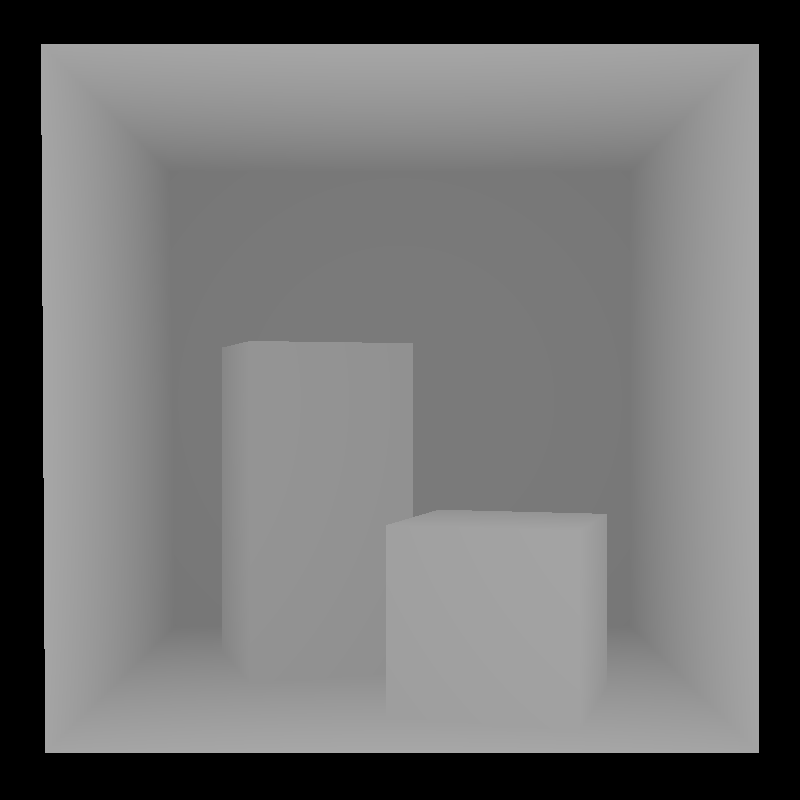
\includegraphics[width=0.38\textwidth]{images/box_render_distance.png}
    \caption{Ukázka vykreslení scény s distance shadingem.}
\end{figure}

\begin{figure}[H]
    \centering
    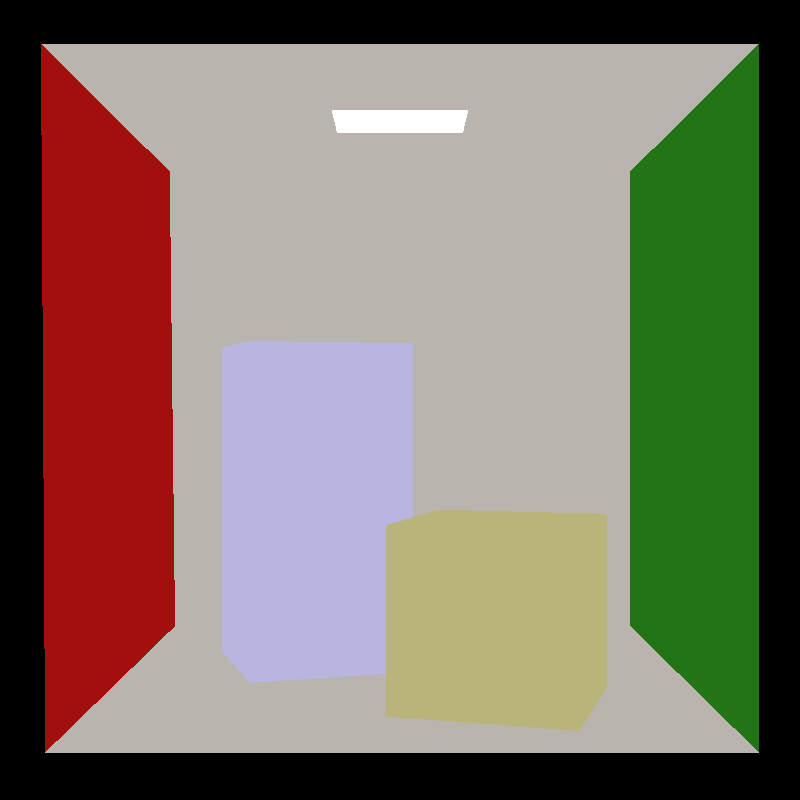
\includegraphics[width=0.38\textwidth]{images/box_render_diffusion.png}
    \caption{Ukázka vykreslení scény s difúzním osvětlením.}
\end{figure}

\begin{figure}[H]
    \centering
    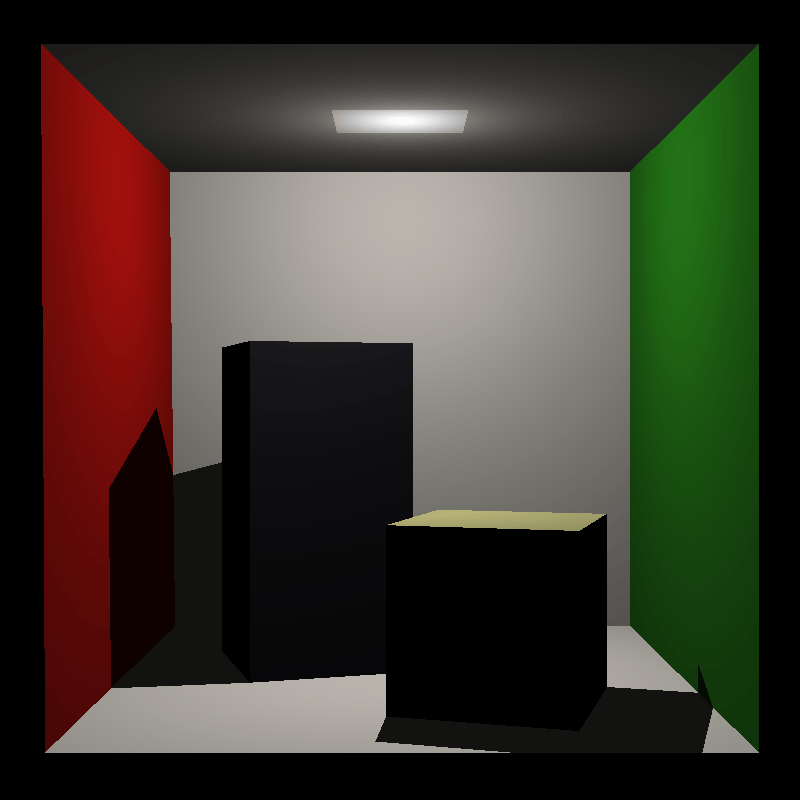
\includegraphics[width=0.38\textwidth]{images/box_render_blinn-phong_shadows.png}
    \caption{Ukázka vykreslení scény s Blinn-Phong osvětlením a stíny.}
\end{figure}

\begin{figure}[H]
    \centering
    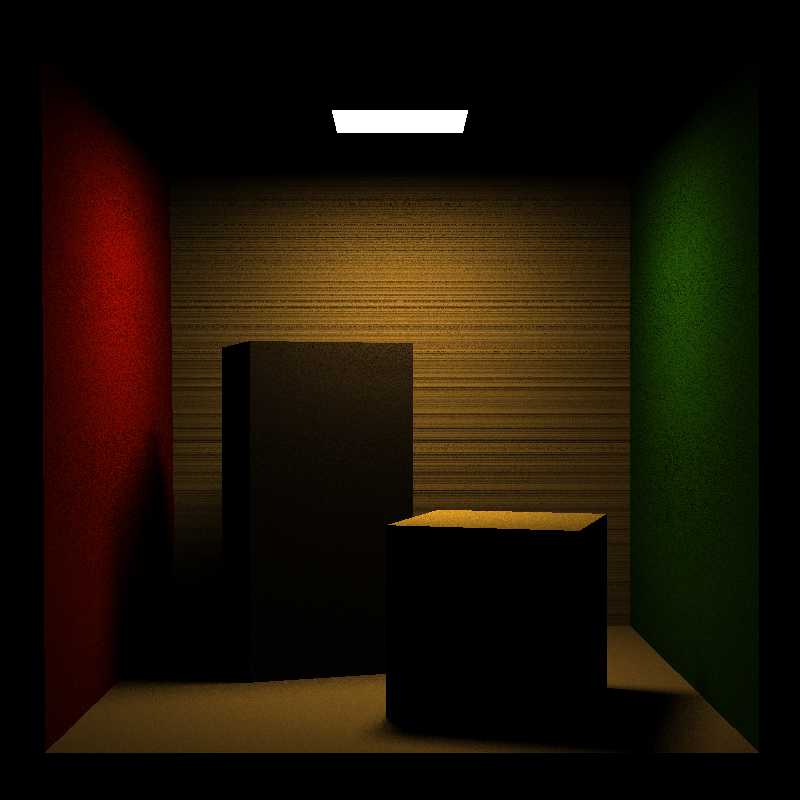
\includegraphics[width=0.38\textwidth]{images/box_render_area_lights.png}
    \caption{Ukázka vykreslení scény s plošným světlem.}
\end{figure}

\begin{figure}[H]
    \centering
    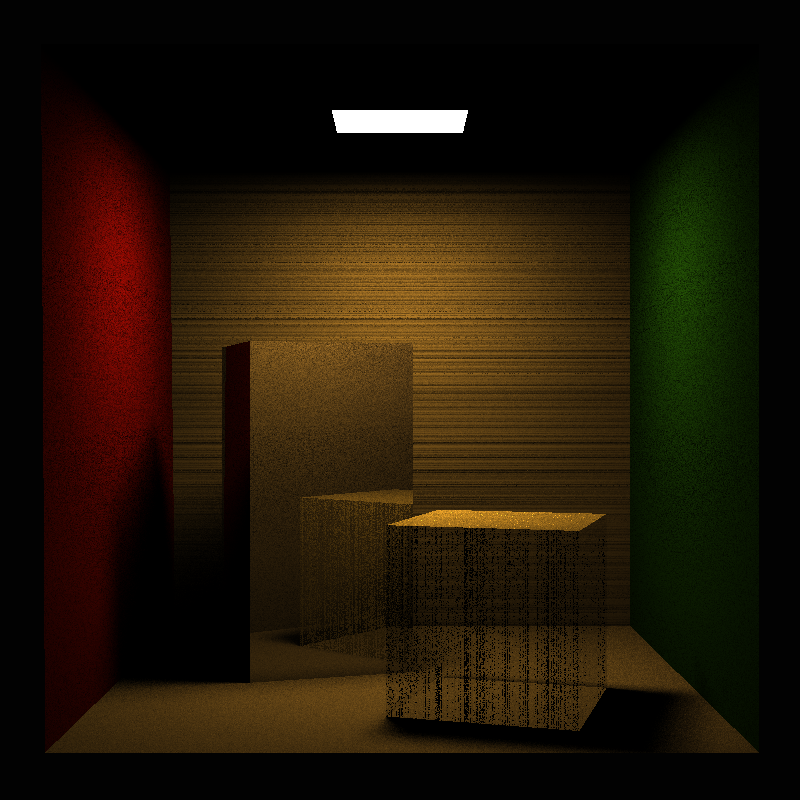
\includegraphics[width=0.38\textwidth]{images/box_render_reflection_refraction.png}
    \caption{Ukázka vykreslení scény s odrazem a lomem světla.}
\end{figure}

\begin{figure}[H]
    \centering
    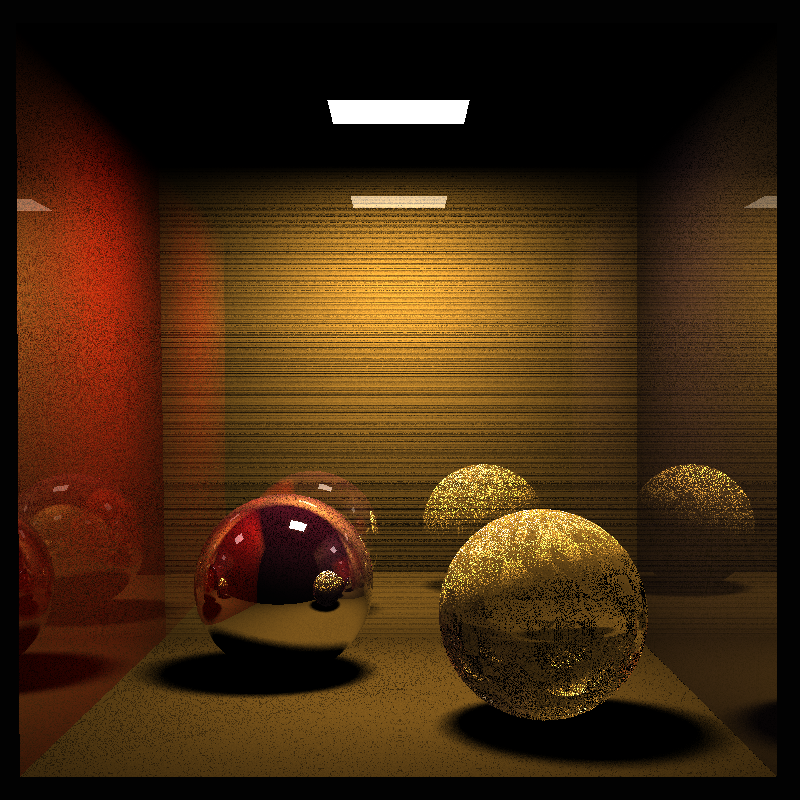
\includegraphics[width=0.38\textwidth]{images/sphere_render_reflection_refraction_walls.png}
    \caption{Ukázka vykreslení scény s odrazem a lomem světla na zrcadlových stěnách.}
\end{figure}

\begin{figure}[H]
    \centering
    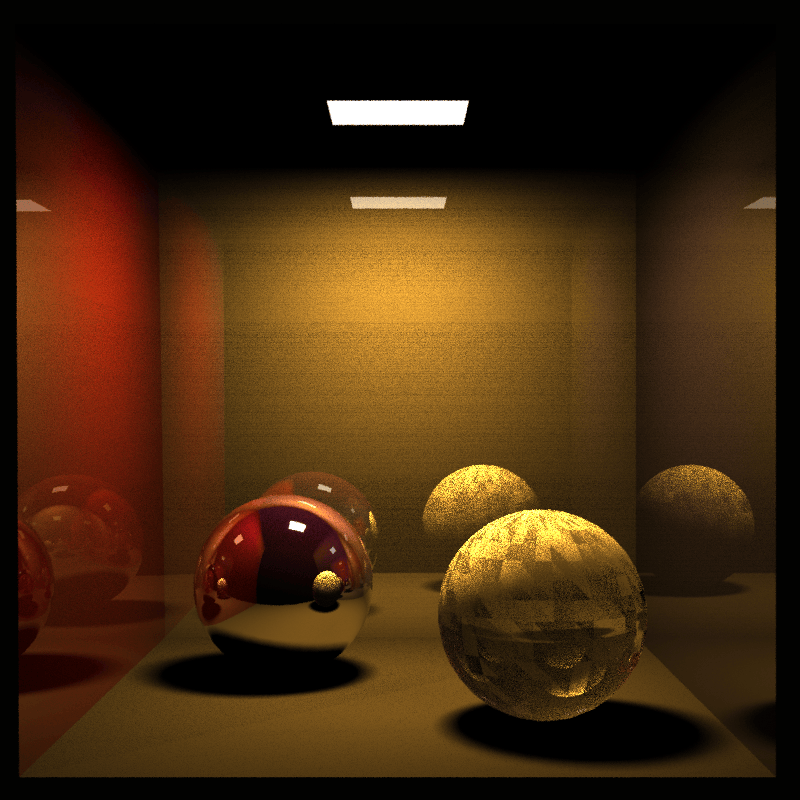
\includegraphics[width=0.38\textwidth]{images/sphere_render_sampling_10.png}
    \caption{Ukázka vykreslení scény s fuzzysamplingem (10~vzorků na pixel).}
\end{figure}

%================================================================================

\section{Implementace}

Veškerá implementace je dostupná na fakultním \href{https://gitlab.fit.cvut.cz/votruja6/pg1-raytracer#}{GitLabu} a mém \href{https://github.com/MasterVotr/PG1-raytracer}{GitHubu}.

Více informací o kompilaci, konfiguraci a spuštění naleznete v~souboru README samotného repozitáře.

%================================================================================

\section{Závěr}

Tato semestrální práce prokázala schopnost optimalizovat výkon raytraceru pomocí akcelerační datové struktury octree a implementace na GPU. Implementace základního octree vedla k~významnému zrychlení traverzace scény a~snížení počtu kolizí mezi paprsky a~trojúhelníky. Parametrickou variantu octree se mi bohužel nepodařilo implementovat, což je škoda, protože by mohla přinést další zlepšení výkonu. implementace na GPU umožnila využít paralelní zpracování a~výrazně zrychlit renderování scény. Výsledky měření ukázaly, že GPU verze raytraceru je schopna vykreslit scénu mnohem rychleji než CPU verze s octree.

Další rozšíření raytraceru by mohlo zahrnovat implementaci dalších akceleračních struktur, jako jsou BVH (Bounding Volume Hierarchy) nebo kd-stromy, které by mohly dále zlepšit výkon při renderování složitějších scén.

\section{Použitá literatura}
\begin{itemize}
    \item Přednášky a materiály z předmětu NI-PG1.
    \item Přednášky a materiály z předmětu NI-GPU.
    \item \textit{An Efficient Parametric Algorithm for Octree Traversal} - Revelles et al.
    \item \texttt{tinyobjloader} - Knihovna pro načítání \texttt{.obj} souborů.
    \item \texttt{nlohmann/json} - Knihovna pro práci s~JSON v~C++.
    \item Dokumentace k C++ standardu a knihovnám.
    \item Dokumentace ke CUDA knihovně.
\end{itemize}


\end{document}
